\section{Conditional weights for the cyclic coordinate schedule}
\label{cycles:section}

The deterministic coordinate schedule admits estimates that do not use an
auxiliary change to random directions. We first give several two-sweep
estimates for arbitrary initial available sets and signed weights. They
yield uniform mixing of
any prescribed list omitting a fixed positive fraction of the cards.
We then track the bitwise difference of two conditional weights. This
autocorrelation gives predictable marginal caps in both coordinate orders;
a two-sided Fourier transfer turns those caps into a $2052d$ bound.

Throughout this section $n=2^d$, $V=\mathbb F_2^d$, and $G=\Sym(V)$.
A \emph{sweep} means the $d$ consecutive coordinate layers
$1,\ldots,d$ in the rotating frame of
\eqref{eq:frames:cyclic}. At a sweep boundary this frame agrees with the
physical position frame. The arguments also hold after any permutation
of the coordinate order, including its reversal. All norms on real
vectors on $V$ below use counting measure.

\subsection{Signed weights on the available set}
\label{cycles:weights}

Let $F\subseteq V$ be a moving set of available positions and put
$h=\one_F$. Attach a real vector $f$ supported on $F$. A coordinate layer
updates each matching pair as follows: with two available endpoints, replace
their weights by their average; with one available endpoint, place its flag
and weight at one of the two endpoints with equal probabilities; with
no available endpoint, leave both weights zero. The choices on distinct pairs
are independent. This preserves $|F|$ and $\sum_x f(x)$, and never
increases $\|f\|_2^2$. Write $A_j$ for ordinary averaging across coordinate
$j$, and $B_i=A_i\cdots A_1$, with $B_0=I$. Conditional on the past,
\begin{equation}\label{cycles:mean-update}
 \E(f_{\rm new}\mid h,f)=A_jf,\qquad
 \E(h_{\rm new}\mid h,f)=A_jh,\qquad
 \E(f_{\rm new}^2\mid h,f)\le A_j(f^2)
\end{equation}
pointwise. The first two identities follow by inspecting the three pair
types. For the last, two weights at available endpoints satisfy
$((a+b)/2)^2\le(a^2+b^2)/2$, and the other cases are equalities.

This process includes the centered conditional distribution of one card
after the trajectories of several other cards have been exposed. Write $X_t(a)$ for the location of the card started at $a$ in the
cyclic coordinate frame. More precisely, if $j$ cards are observed through time $t$, let $\mathcal F_t$
be their trajectory field, $F_t$ their complement, and $a$ a further
initial label. Then
\begin{equation}\label{cycles:conditional-weight}
 f_t(x)=\Pr(X_t(a)=x\mid\mathcal F_t)
               -\frac{\one_{F_t}(x)}{n-j}
\end{equation}
has exactly the transition law above by
Lemma~\ref{lem:marginal-averaging}, applied with the observed cards as
blockers. The same rule transports the uniform vector on the available
set. The process is adapted to $\mathcal F_t$; it is not obtained by
conditioning its transitions on a future event. Its initial energy is
at most one. The real weights considered here have broader scope than
this application: they may be any deterministic signed vector supported
on the initial available set. The contraction statements below retain
that scope, with their stated zero-sum hypotheses.

\begin{lemma}[From signed-weight energy to list mixing]
\label{cycles:list}
Fix $p\in(0,1)$ and an integer $R\ge1$. Suppose every deterministic
zero-sum weight configuration on an available set with $|F|\ge pn$ satisfies
$\E\|f_{2d}\|_2^2\le \kappa_d\|f_0\|_2^2$ over two sweeps.
After $2R$ sweeps the images of any fixed ordered list of at most
$(1-p)n$ distinct initial labels have total-variation distance at most
\begin{equation}\label{cycles:list-error}
 \frac12 n^{3/2}\kappa_d^{R/2}
\end{equation}
from the uniform distinct-position list.
\end{lemma}
\begin{proof}
Successive conditioning at two-sweep boundaries gives
$\E\|f_{2Rd}\|_2^2\le \kappa_d^R$ for the centered conditional law of each
next card, exposing all preceding cards. There are always at least $pn$
available positions. Cauchy--Schwarz bounds its expected conditional
variation distance by $\frac12\sqrt{n\kappa_d^R}$. Conditioning on the preceding
endpoints alone can only decrease this expectation: the uniform reference
on available positions is already measurable from those endpoints, and the
conditional law is the conditional expectation of the path-conditioned
law. Finally interpolate between joint laws with a true prefix of length
$j$ and uniform sampling without replacement thereafter. Consecutive
laws differ by the conditional error at the next card, averaged under
the actual prefix law. Summing at most $n$ such errors proves the bound.
\end{proof}

\subsection{Coarse averaging and the energy of a second sweep}
\label{cycles:coarse}

We first give an independent noise-based argument. It controls coarse
block averages by a martingale expansion, then uses the remaining
coordinates of a second sweep to remove energy. The following subsection
will obtain sharper block moments from the transverse fibers instead.

\begin{proposition}[Coarse-energy contraction]
\label{cycles:coarse-prop}
For $|F|\ge n/8$ and $\sum_xf(x)=0$, the signed-weight process satisfies,
for all sufficiently large $d$,
\begin{equation}\label{cycles:coarse-contraction}
 \E\|f_{2d}\|_2^2\le n^{-1/256}\|f_0\|_2^2.
\end{equation}
Consequently $4096$ sweeps mix every fixed list of at most $7n/8$ cards
with variation error at most $\frac12 n^{-5/2}$.
\end{proposition}
\begin{proof}
Let $m=\lfloor3d/4\rfloor$ and $p=|F_0|/n$. At layer $j$ of a sweep,
\[
 f_j=A_jf_{j-1}+\xi_j.
\]
Conditional on the past, $\xi_j$ is the sum, over pairs
$\{u,v\}$ with exactly one available endpoint $u$, of independent centered vectors
$\pm f_{j-1}(u)(e_u-e_v)/2$. Here $e_x$ denotes the unit vector at a
position $x$. Expanding the entire sweep, the centered noise terms at
different times are orthogonal in second moment, even after applying
deterministic averaging operators. Moreover
$\|B_m(e_u-e_v)\|_2^2\le2\cdot2^{-m}$, and all coordinate averages
commute. Since $B_df_0=0$, and writing $f^*,h^*$ for the output,
\begin{equation}\label{cycles:coarse-moments}
 \E\|B_mf^*\|_2^2\le d2^{-m}\|f_0\|_2^2,\qquad
 \E\|B_mh^*-p\one\|_2^2\le d2^{-m}n.
\end{equation}
For the second inequality use the same expansion for flags and
$\|h_0\|_2^2=pn\le n$. Energy monotonicity bounds each layer's sum of
squared noise coefficients by the initial energy.

A level-$m$ block varies in coordinates $1,\ldots,m$. If one such block
has a fraction of available positions below $1/16$, the second squared norm in
\eqref{cycles:coarse-moments} is at least $2^m/256$.
Thus the event $\mathcal G$ that all these blocks have density at least
$1/16$ satisfies
$\Pr(\mathcal G^c)\le256dn2^{-2m}$.

Condition on the output of sweep one. Before coordinate $j$ of sweep
two, distinct level-$(j-1)$ blocks have used disjoint fresh coins.
In particular the two endpoints $x,y$ of the next pair have independent
flag-weight data, whose means are the entries of
$B_{j-1}h^*,B_{j-1}f^*$. Their energy loss is exactly
\[
 \frac12\bigl(h(y)f(x)^2+h(x)f(y)^2-2f(x)f(y)\bigr).
\]
On $\mathcal G$, for $j>m$ both flag means are at least $1/16$.
The sum of the expected cross products over the pairs is at most
$\frac12\|B_{j-1}f^*\|_2^2\le\frac12\|B_mf^*\|_2^2$.
The conditional expected energy therefore contracts by $31/32$ at each
such step, with additive term $\frac12\|B_mf^*\|_2^2$.
Iterating this recurrence, and using monotonicity on $\mathcal G^c$,
gives
\begin{equation}\label{cycles:coarse-factor}
 \E\|f_{2d}\|_2^2\le
 \left((31/32)^{d-m}+16d2^{-m}+256dn2^{-2m}\right)\|f_0\|_2^2.
\end{equation}
Each term is $o(n^{-1/256})$: for the first use
$(31/32)^{d-m}\le e^{-d/128}$, while the others have powers at least
$3/4$ and $1/2$, up to polynomial factors in $d$.
This proves \eqref{cycles:coarse-contraction}. Iterating $2048$
two-sweep blocks gives energy $n^{-8}$, and Lemma~\ref{cycles:list}
gives the stated marginal error.
\end{proof}

\subsection{Block statistics and the exact merge}\label{cycles:block-core}

A level-$j$ block fixes coordinates $j+1,\ldots,d$ and varies the
first $j$; write $\mathcal B_j$ for this partition into blocks of size
$2^j$. Its transverse fibers fix the first $j$ coordinates and vary
the rest. The first $j$ layers act inside the blocks. Once those layers
are fixed, the remaining layers act independently in the transverse
fibers. Writing a site as $(a,b)$, the prefix $a$ indexes the
fibers and the suffix $b$ indexes the blocks. Each block meets each
fiber once, as in Figure~\ref{cycles:transverse-figure}. This crossing of the two
partitions gives both a small signed block sum and a concentrated
available count at the end of a sweep.

\begin{figure}[ht]
\centering
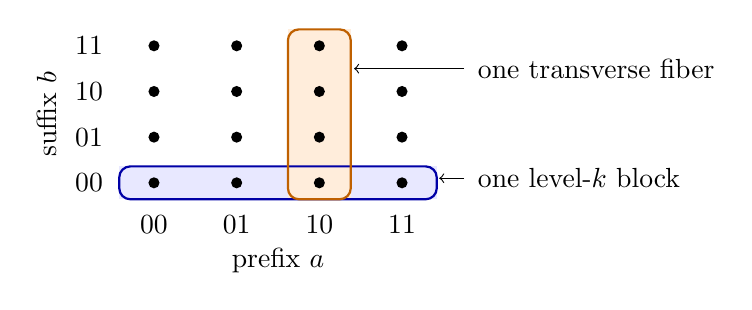
\begin{tikzpicture}[x=1.05cm,y=.58cm]
 \fill[blue!9] (-.42,-.36) rectangle (3.42,.36);
 \fill[orange!14] (1.62,-.36) rectangle (2.38,3.36);
 \draw[blue!65!black,thick,rounded corners] (-.42,-.36) rectangle (3.42,.36);
 \draw[orange!75!black,thick,rounded corners] (1.62,-.36) rectangle (2.38,3.36);
 \foreach \x in {0,1,2,3} {
   \foreach \y in {0,1,2,3} {\fill (\x,\y) circle (2pt);}
 }
 \node[below] at (0,-.5) {$00$};
 \node[below] at (1,-.5) {$01$};
 \node[below] at (2,-.5) {$10$};
 \node[below] at (3,-.5) {$11$};
 \node[left] at (-.5,0) {$00$};
 \node[left] at (-.5,1) {$01$};
 \node[left] at (-.5,2) {$10$};
 \node[left] at (-.5,3) {$11$};
 \node at (1.5,-1.7) {prefix $a$};
 \node[rotate=90] at (-1.3,1.5) {suffix $b$};
 \node[right,align=left] at (3.8,.1) {one level-$k$ block};
 \node[right,align=left] at (3.8,2.5) {one transverse fiber};
 \draw[->] (3.75,.1)--(3.45,.1);
 \draw[->] (3.75,2.5)--(2.42,2.5);
\end{tikzpicture}
\caption{The case $d=4$, $k=2$. The first $k$ layers act within
the horizontal blocks. After those layers are fixed, the remaining
layers evolve independently in the vertical fibers. Each horizontal
block receives one final site from every fiber.}
\label{cycles:transverse-figure}
\end{figure}

\begin{lemma}[Statistics after one sweep]\label{sweeps:block-statistics}
Fix $0<\varepsilon\le1$. Start a sweep from deterministic $(F,f)$
with $|F|\ge\varepsilon n$, $\sum_xf(x)=0$, and energy
$E_0=\|f\|_2^2$. Denote its output by $(F^*,f^*)$ and write
$S_B=\sum_{x\in B}f^*(x)$ and $m_B=|F^*\cap B|$. For
$B\in\mathcal B_j$, of size $s=2^j$,
\begin{equation}\label{sweeps:block-variance}
 \E S_B^2\le(s/n)E_0,\qquad
 \Pr(m_B<\varepsilon s/2)\le e^{-\varepsilon^2s/2}.
\end{equation}
The second bound can alternatively be replaced by
$\exp[-(1/2-e^{-1})\varepsilon s]$.
\end{lemma}
\begin{proof}
Condition on the configuration after coordinate $j$. The remaining
layers use independent switch arrays in the $s$ transverse fibers,
each of size $n/s$. The final entry at the one site where a fiber
meets $B$ has conditional mean equal to that fiber's mean signed
weight and second moment at most its mean squared weight, by
\eqref{cycles:mean-update}. The sum of these means is
$(s/n)\sum_x f(x)=0$. Independence between fibers therefore bounds
the conditional second moment of $S_B$ by $(s/n)$ times the energy
at the conditioning time, which is at most $E_0$.

The availability indicators at those $s$ sites are likewise independent
under this conditioning. Their total mean is
$\mu=|F|s/n\ge\varepsilon s$. Hoeffding's inequality
(Lemma~\ref{lem:concentration}) bounds a downward deviation of at least
$\varepsilon s/2$ by $e^{-\varepsilon^2s/2}$. Alternatively, for their
sum $J$, independence gives
$\E e^{-J}\le e^{-(1-e^{-1})\mu}$, and hence
$\Pr(J<\mu/2)\le e^{-(1/2-e^{-1})\mu}$.
\end{proof}

The next identity describes how a sweep uses these block statistics.
Its inputs are deterministic at the start of that sweep; no independence
between blocks of a preceding sweep's output is required.

\begin{lemma}[The block-merging identity]\label{sweeps:merge}
Start a sweep deterministically. Suppose two sibling blocks have size
$s$, available counts $m_0,m_1$ and signed sums $S_0,S_1$. Let
$\overline E_0,\overline E_1$ be their expected energies after their
internal coordinates have been updated. The expected energy after
their merging coordinate is
\begin{equation}\label{sweeps:merge-eq}
 (1-m_1/(2s))\overline E_0+
 (1-m_0/(2s))\overline E_1+S_0S_1/s.
\end{equation}
\end{lemma}
\begin{proof}
The child blocks use independent switch arrays before merging.
The averaging identities in \eqref{cycles:mean-update} give, at each
site of child $i$, expected availability $m_i/s$ and expected signed
weight $S_i/s$. No equality between the individual sites' second
moments is needed. On an edge with weights $a,b$ and availability
indicators $q_a,q_b$, the energy loss is
$(q_ba^2+q_ab^2-2ab)/2$. Independence across children and summation
over their $s$ paired sites give expected loss
\[
 \frac{m_1\overline E_0+m_0\overline E_1-2S_0S_1}{2s},
\]
which proves the identity.
\end{proof}

\subsection{Transverse block sampling and zero block sums}
\label{cycles:zero-block}

The next argument first removes the small component that is constant on
the available positions of each block. The remaining component has zero expected
weight at each site in the latter half of the next sweep.

\begin{proposition}[Blockwise centered contraction]
\label{cycles:centered-prop}
For $p=1/16$, arbitrary $|F|\ge pn$, and zero-sum $f$, two sweeps
satisfy \eqref{cycles:coarse-contraction}. After $2048$ sweeps every
fixed list of at most $15n/16$ labels has variation error at most
$\frac12 n^{-1/2}$.
\end{proposition}
\begin{proof}
Put $k=\lfloor d/2\rfloor$, $L=2^k$, and $M=2^{d-k}$, and denote
the first-sweep output by $(F^*,f^*)$. Sum the moment bound in
Lemma~\ref{sweeps:block-statistics} over the $M$ level-$k$ blocks.
Its exponential tail, using $1/2-e^{-1}>1/8$, and a union bound give
\begin{equation}\label{cycles:transverse}
 \Pr(\mathcal G^c)\le M e^{-pL/8},\qquad
 \E\sum_B S_B^2\le\|f_0\|_2^2,\qquad
 \mathcal G=\{|F^*\cap B|\ge pL/2\text{ for every }B\}.
\end{equation}
For each first-sweep output in $\mathcal G$, write $f^*=u+w$, where
$u$ has constant value $S_B/|F^*\cap B|$ on each $F^*\cap B$.
This is an orthogonal decomposition, $w$ has zero sum in each block, and
\[
 \|u\|_2^2=\sum_B\frac{S_B^2}{|F^*\cap B|}
       \le\frac{2}{pL}\sum_BS_B^2.
\]
Run $w$ through the second sweep. After the first $j\ge k$ coordinates,
its expected value at each site is zero and the probability of availability is at
least $p/2$. Different level-$j$ blocks have evolved independently, so
at the next merging pair the expected product of weights is zero.
In the energy-loss formula the opposite flag multiplies each squared
weight independently, with expectation at least $p/2$. The expected
energy hence contracts by $1-p/4$ for each of the last $d-k$ layers.
The $u$ component cannot increase in norm. Using
$\|u_{\rm out}+w_{\rm out}\|_2^2\le2\|u_{\rm out}\|_2^2+
2\|w_{\rm out}\|_2^2$, and monotonicity outside $\mathcal G$, proves
\begin{equation}\label{cycles:centered-factor}
 \E\|f_{2d}\|_2^2\le
 \left(Me^{-pL/8}+2(1-p/4)^{d-k}+\frac4{pL}\right)\|f_0\|_2^2.
\end{equation}
Here $(1-p/4)^{d-k}\le e^{-d/128}$, and the other terms decay faster
than $n^{-1/256}$. Thus their sum is at most $n^{-1/256}$ eventually.
After $1024$ two-sweep blocks the energy is at most $n^{-4}$;
Lemma~\ref{cycles:list} proves the conclusion.
\end{proof}

\subsection{A recurrence for all large blocks}
\label{cycles:merge}

One can retain the block sums in the recurrence instead of separating
them off. This yields a useful contraction for every fixed density of available positions.

\begin{proposition}[Multilevel energy contraction]
\label{cycles:merge-prop}
Fix $p\in(0,1)$ and set $r=\lfloor d/2\rfloor$. For arbitrary
$|F|\ge pn$ and zero-sum $f$, two sweeps satisfy
\begin{equation}\label{cycles:merge-factor}
 \E\|f_{2d}\|_2^2\le
 \left((1-p/4)^{d-r}+2^{-r}
             +2^{d-r}e^{-p2^r/8}\right)\|f_0\|_2^2.
\end{equation}
In particular the factor is at most $n^{-\gamma_p}$ eventually, where
$\gamma_p=-\frac14\log_2(1-p/4)>0$.
It is also at most $n^{-p/16}$ eventually.
\end{proposition}
\begin{proof}
For level-$i$ blocks $B$ of size $2^i$, define
\[
 S_i(f)=2^{-i}\sum_B\left(\sum_{x\in B}f(x)\right)^2.
\]
The block statistics of Lemma~\ref{sweeps:block-statistics}, now
applied at every level $i$, give
\begin{equation}\label{cycles:all-level-moments}
 \E S_i(f^*)\le2^{-i}\|f_0\|_2^2,\qquad
 \Pr\{\text{some level-$r$ block has density below }p/2\}
 \le2^{d-r}e^{-p2^r/8}.
\end{equation}
Indeed each level-$i$ block meets every transverse fiber once.
Lemma~\ref{sweeps:block-statistics}, summed over the $n/2^i$ blocks,
gives the first bound. For the second, its proof gives a sum of independent
availability indicators of mean at least $p2^r$; the Bernoulli lower-tail
bound used in \eqref{cycles:transverse} and a union bound suffice.

Condition now on $f^*,F^*$ with all level-$r$ block densities at
least $p/2$. Their unions have the same lower density bound. In the
second sweep, Lemma~\ref{sweeps:merge} therefore multiplies each
child energy by at most $1-p/4$. Its signed cross term is bounded
using $2S_{B_0}S_{B_1}\le S_{B_0}^2+S_{B_1}^2$. Summing over
merges of level-$i$ blocks, and writing $E_i$ for the energy after
$i$ layers of this sweep, gives
\[
 \E(E_{i+1}\mid f^*,F^*)
 \le(1-p/4)\E(E_i\mid f^*,F^*)+\frac12S_i(f^*),
 \qquad r\le i<d.
\]
Iterate, discard the contraction factors on the nonnegative additive
terms, use \eqref{cycles:all-level-moments}, and use pathwise monotonicity
on the excluded event. The geometric sum
$\frac12\sum_{i=r}^{d-1}2^{-i}\le2^{-r}$ proves
\eqref{cycles:merge-factor}. Its first term is at most $n^{-2\gamma_p}$;
the other terms are $O(n^{-1/2})$ and exponentially small in $\sqrt n$,
respectively. Since $\gamma_p<1/2$, their sum is at most
$n^{-\gamma_p}$ eventually. Also the first term is at most
$e^{-pd/8}=n^{-p/(8\log2)}$, whose exponent exceeds $p/16$,
proving the alternative assertion.
\end{proof}

\begin{remark}[Translation symmetry and a variant of the error bound]
\label{cycles:invariance}
A completed block also has a distributional symmetry. After its $i$
internal coordinates have been processed, its flag-weight law is
invariant under bit translations of those coordinates. Inductively,
old-coordinate translations permute the fresh matching edges, while
flipping the new coordinate preserves the independent fair placements
and the equal outputs of averaging. The symmetry makes each site's
second moment the expected block energy divided by $2^i$.

This supplies another derivation of \eqref{sweeps:merge-eq}, although
the first-moment proof of Lemma~\ref{sweeps:merge} does not require it.
It also permits the following version of the multilevel estimate.
For the first-sweep output,
$\E\sum_{B\in\mathcal B_i}S_B^2\le\|f_0\|_2^2$ and
$\Pr(m_B<p2^i/2)\le e^{-p2^i/8}$. A union bound over every level
$r\le i<d$, followed by the exact merge identity and
$2S_{B_0}S_{B_1}\le S_{B_0}^2+S_{B_1}^2$, gives
\begin{equation}\label{cycles:invariance-factor}
 (1-p/4)^{d-r}+2^{-r}+dn e^{-p2^r/8}\le n^{-p/16}
\end{equation}
for large $d$. This is a slightly weaker error term than
\eqref{cycles:merge-factor}; both bounds condition on the full
first-sweep output before using fresh, independent second-sweep blocks.
\end{remark}

\subsection{Negative correlation and block variances}
\label{cycles:negative}

The last two-sweep argument obtains first-sweep moments from pairwise
negative correlation of card locations. It then contracts variance
about the mean on the available positions of each block.

\begin{proposition}[Variance contraction from pairwise correlation]
\label{cycles:negative-prop}
Fix $\delta\in(0,1]$. For arbitrary $|F|\ge\delta n$ and zero-sum $f$,
there is $a=a(\delta)>0$ such that two sweeps satisfy
$\E\|f_{2d}\|_2^2\le n^{-a}\|f_0\|_2^2$ for all large $d$.
One may take $a=-\frac18\log_2(1-\delta/4)$.
\end{proposition}
\begin{proof}
For a level-$s$ block $B$ put $p_B=|B|/n$. Membership in $B$
means that the last $d-s$ output bits equal its prescribed suffix.
Every card has membership probability $p_B$. To compare two distinct
cards, let $i$ be their largest initially differing coordinate. Before
layer $i$, they use distinct switches, so their output bits are
independent fair bits. At layer $i$ they use one switch exactly when
their earlier output prefixes agree; that switch forces opposite
outputs. After layer $i$ their prefixes are distinct, and they use
distinct switches for the rest of the sweep.

If $i\le s$, the only possible shared switch is in an unconstrained
coordinate. All prescribed suffix bits are then sampled at distinct
switches, and joint membership has probability $p_B^2$. If $i>s$,
condition on both cards having the prescribed outputs at coordinates
$s+1,\ldots,i-1$. Their first $s$ outputs remain independent uniform
strings, so their prefixes agree with probability $2^{-s}$. On this
event joint membership is impossible at layer $i$; off it both
prescribed outputs occur with probability $1/4$. The remaining
prescribed bits are again sampled at distinct switches. Thus joint
membership has probability $p_B^2(1-2^{-s})\le p_B^2$.
In either case the membership indicators have nonpositive covariance.

Let $C$ be the covariance matrix of the membership indicators of all $n$
initial labels. Their sum is the fixed number $|B|$, so $C$ has zero row
sums. Its off-diagonal entries are nonpositive, and its diagonal is at
most $p_B$. Therefore
\[
 v^TCv=\sum_{x<y}(-C_{xy})(v_x-v_y)^2
 \le2p_B\sum_xv_x^2.
\]
Let $h_B$ count the cards that start in $F_0$ and end in $B$, and let
$u_B$ be the sum of averaged loads there. It follows that
\begin{equation}\label{cycles:negative-moments}
 \E h_B=p_B|F|,\qquad
 \operatorname{Var}(h_B)\le p_B|F|,\qquad
 \E u_B^2\le2p_B\|f_0\|_2^2.
\end{equation}
For the last estimate, give the card initially at $a\in F_0$ the
deterministic signed weight $f_0(a)$, and give every observed card,
initially outside $F_0$, weight zero. If $g_t$ is the actual position
permutation, the transported load is
$\widetilde f_t(x)=f_0(g_t^{-1}x)$, with $f_0$ extended by zero.
Fix a feasible history $\mathcal H$ of all observed-card trajectories
through the first sweep. Lemma~\ref{lem:marginal-averaging} leaves the
unvisited switches independent and fair, including an earlier unvisited
switch when later observed paths are specified. The additional step here
is to apply that conditional-flow rule to arbitrary signed loads.
At a pair with two available inputs, averaging that unvisited fair coin
averages the two incoming expected loads. At a pair with one available input,
the observed trajectory determines its available output, so its load is
transported to that output. Induction over layers, using linearity for
the signed weights, therefore gives
\begin{equation}\label{cycles:signed-load-jensen}
 f_t(x)=\E[\widetilde f_t(x)\mid\mathcal H],\qquad
 u_B=\E\!\left[\sum_{a\in F_0}f_0(a)
                    \mathbf1_{\{g_d(a)\in B\}}\,
                    \middle|\,\mathcal H\right].
\end{equation}
Each initial label has probability $p_B$ of ending in $B$, and
$\sum_a f_0(a)=0$, so the unaveraged sum has mean zero and second moment
$f_0^TCf_0\le2p_B\|f_0\|_2^2$. Conditional Jensen proves the asserted
bound for $u_B$ for every signed initial load.

If $\delta=1$, every position is available, so one sweep applies all
coordinate averages and sends the zero-sum vector to zero. The list
statement then concerns the empty list and is exact. For the remaining
argument assume $0<\delta<1$.

Put $s_0=\lfloor3d/4\rfloor$. Chebyshev gives probability at most
$4/(\delta2^s)$ that a fixed level-$s$ block has
$h_B<\delta2^s/2$. There are $n/2^s$ such blocks. Summing over
$s\ge s_0$ bounds the failure probability by
$O_\delta(n2^{-2s_0})=O_\delta(n^{-1/2})$.
Condition on a first-sweep output outside that event. At a second-sweep
merge of children $L,R$ of size $m=2^{s-1}$, write
$b_L=u_L/h_L$, $b_R=u_R/h_R$ for their means over available positions.
Let $V_L,V_R$ be their expected squared deviations from these means
immediately before the merge, and $V_B$ the corresponding parent
quantity. Subtracting the parent mean energy from the common
block-merging identity, Lemma~\ref{sweeps:merge}, gives
\begin{align}\label{cycles:variance-merge}
 V_B={}&\left(1-\frac{h_R}{2m}\right)V_L+
 \left(1-\frac{h_L}{2m}\right)V_R\notag\\
 &+\left(1-\frac{h_L+h_R}{2m}\right)
       \frac{h_Lh_R}{h_L+h_R}(b_L-b_R)^2.
\end{align}
To verify it, the premerge total energy is
$V_L+V_R+h_Lb_L^2+h_Rb_R^2$; the expected loss is
$[h_RV_L+h_LV_R+h_Lh_R(b_L-b_R)^2]/(2m)$.
Subtract the parent mean term
$(h_Lb_L+h_Rb_R)^2/(h_L+h_R)$ to obtain the formula.
All denominators are positive on the retained event.

For $s>s_0$ the first two coefficients are at most $1-\delta/4$.
The last term is nonnegative and at most
$u_L^2/h_L+u_R^2/h_R$. Iterating to the root, whose load mean is zero,
bounds the final conditional energy by
\[
 (1-\delta/4)^{d-s_0}\|f_0\|_2^2+
 \sum_{s=s_0}^{d-1}\frac{2}{\delta2^s}
                   \sum_{|B|=2^s}u_B^2.
\]
For each level \eqref{cycles:negative-moments} bounds the expectation
of the inner sum by $2\|f_0\|_2^2$. Use monotonicity on the discarded
event. The resulting two-sweep factor is
\begin{equation}\label{cycles:negative-factor}
 (1-\delta/4)^{d-s_0}
       +O_\delta(2^{-s_0})+O_\delta(n2^{-2s_0}).
\end{equation}
Its leading term is at most $n^{-2a}$ for the stated $a$, and the two
other terms are $O_\delta(n^{-3/4})$ and $O_\delta(n^{-1/2})$.
This proves the claim. By Lemma~\ref{cycles:list}, any fixed
$R$ with $aR>3$ now suffices for the asserted large-list mixing.
\end{proof}

\subsection{From the two-sweep estimates to the full deck}
\label{cycles:two-sweep-completion}

The five energy estimates give different quantitative parameters for the
abstract Fourier transfers, even when two total times coincide. We record the exact
substitutions. For disjoint block subgroups $H_i=\Sym(D_i)$, a
subprobability $\nu$ satisfying $\nu(gH_i)\le B/[G:H_i]$ has
\begin{equation}\label{cycles:orbit-bound}
 \|\widehat\nu(\rho)\|_{\op}
 \le\sqrt{rBC_s}\,D^{-(1-(s+2)/r)/2},
\end{equation}
by Proposition~\ref*{l-l:orbit-span} of \cite{partialFourier}. Here $r$ is the
number of blocks, $D=\dim\rho$, and $C_s$ is the reciprocal-degree
constant defined in Section~\ref{mart:applications}. That companion
also proves two distinct central-projection bounds in
Proposition~\ref*{l-l:central-projector-operator} of~\cite{partialFourier}. For a probability
$\eta$ with the same caps they are
\begin{align}
 \|\widehat\eta(\rho)\|_{\op}
 &\le BC_s\sqrt r\,D^{-1/2+(s+2)/r},\label{cycles:projector-op-one}\\
 \|\widehat\eta(\rho)\|_{\op}
 &\le B\sqrt{rC_s}\,D^{-1/2+(s+2)/(2r)}.\label{cycles:projector-op-two}
\end{align}
The first uses pointwise character control; the second uses cosetwise
spectral projection. Both require one simultaneous cap for all the
subgroups. Lemma~\ref*{l-l:trim} of~\cite{partialFourier} supplies it with the mass costs stated
in Section~\ref{mart:applications}.

\begin{proposition}[Full-deck bounds from two sweeps]
\label{cycles:two-sweep-bounds}
Each row of Table~\ref{cycles:transfer-table} gives total-variation
convergence of the full permutation law to uniform as $d\to\infty$,
uniformly over deterministic initial decks.
\end{proposition}

In the table, $r$ counts equal label blocks, $T$ is the length of one
shuffle block, and $\ell$ counts independent shuffle blocks. For the
multilevel row set
\[
 \gamma=-\tfrac14\log_2(127/128),\qquad h=\lceil6/\gamma\rceil.
\]
In the translation row use $R=128\cdot128$. In the negative-correlation
row, $R$ is any fixed integer with $a(1/8)R>3$, where $a$ is from
Proposition~\ref{cycles:negative-prop}. Each displayed Fourier bound is
an operator-norm bound at irreducible degree $D$.

\begingroup
\small
\setlength{\tabcolsep}{4pt}
\renewcommand{\arraystretch}{1.2}
\begin{longtable}{@{}p{.32\linewidth}p{.31\linewidth}r r r@{}}
\caption{Two-sweep inputs and their full-deck substitutions.
The exponent $\kappa$ is $2-2\ell\alpha$ for an operator bound
$K D^{-\alpha}$.}\label{cycles:transfer-table}\\
\toprule
Input and retained measure & Transfer and Fourier bound
 & $\ell$ & $\kappa$ & Total time$/d$\\
\midrule
\endfirsthead
\toprule
Input and retained measure & Transfer and Fourier bound
 & $\ell$ & $\kappa$ & Total time$/d$\\
\midrule
\endhead
\bottomrule
\endfoot
Coarse energy, $T/d=4096$;\newline
$r=8$, probability, cap $2$
&
Orbit, \eqref{cycles:orbit-bound}, $s=1$;\newline
$\sqrt{16C_1}D^{-5/16}$
& $8$ & $-3$ & $32768$\\
Blockwise centered, $T/d=2048$;\newline
$r=16$, subprobability, cap $1$
&
Orbit, \eqref{cycles:orbit-bound}, $s=4$;\newline
$\sqrt{16C_4}D^{-5/16}$
& $16$ & $-8$ & $32768$\\
Multilevel, $p=1/32$, $T/d=2h$;\newline
$r=32$, cap-one subprobability,\newline
then restore uniform mass
&
Orbit, \eqref{cycles:orbit-bound}, $s=8$;\newline
$\sqrt{32C_8}D^{-11/32}$
& $16$ & $-9$ & $32h$\\
Translation symmetry, $p=1/128$,\newline
$T/d=2R$; $r=128$,\newline
probability, cap $4$
&
Pointwise projector,\newline
\eqref{cycles:projector-op-one}, $s=6$;\newline
$4C_6\sqrt{128}D^{-7/16}$
& $16$ & $-12$ & $524288$\\
Negative correlation, $\delta=1/8$,\newline
$T/d=2R$; $r=8$,\newline
probability, cap $3$
&
Cosetwise projector,\newline
\eqref{cycles:projector-op-two}, $s=2$;\newline
$3\sqrt{8C_2}D^{-1/4}$
& $8$ & $-2$ & $16R$\\
\end{longtable}
\endgroup

\begin{proof}
The input marginal errors follow from Lemma~\ref{cycles:list}.
The coarse and centered bounds are those of
Propositions~\ref{cycles:coarse-prop} and \ref{cycles:centered-prop}.
For the multilevel row, Proposition~\ref{cycles:merge-prop} gives
energy $n^{-h\gamma}$ and marginal error
$\varepsilon_n\le\tfrac12n^{(3-h\gamma)/2}=o(1)$.
For translation symmetry, \eqref{cycles:invariance-factor} has exponent
$p/16=1/2048$, so $(p/16)R=8$ and the marginal error is
$\tfrac12n^{-5/2}$. The last row has error
$\tfrac12n^{(3-a(1/8)R)/2}=o(1)$.
Each bound is uniform, so any fixed partition into the indicated
$r$ equal blocks supplies all the complementary marginals.

Use the simultaneous trimming operations of
Section~\ref{mart:applications}. For the first row, excess trimming
followed by normalization gives cap $2$ eventually. For the fourth
and fifth, heavy-coset deletion and normalization give caps $4$ and
$3$. These probability laws are within $o(1)$ of their original block
laws. The second and third rows retain cap-one subprobabilities before
their different completions.

Substituting the table's caps, block counts and reciprocal-degree
parameters in the preceding three transfer formulas gives its Fourier
bounds. The exponents $\kappa$ follow from
$D\|M^\ell\|_{\HS}^2\le D^2\|M\|_{\op}^{2\ell}$.
Their sums tend to zero by the respective reciprocal-degree estimates
at powers $1,4,8,6,2$ in
\cite[Theorem~\ref*{l-l:degree-all-powers}]{partialFourier}.

For the multilevel row, the cap-one construction loses mass
$\delta\le32\varepsilon_n$. Restore it as $\eta=\nu+\delta U_G$.
Every nontrivial Fourier matrix of $\eta$ equals that of $\nu$, so
the table's orbit bound still applies, and
$\|\eta-\mu\|_{\TV}\le\delta=o(1)$ for the original block law $\mu$.
Thus this row, like the first, fourth and fifth, meets the probability
completion of Section~\ref{sec:probability-completion}: the original
law has zero sign expectation, the nearby probability has sign
coefficient $o(1)$, and replacing the fixed number of factors costs
$o(1)$.

The centered row instead convolves the cap-one subprobability itself.
Write $z=\nu(G)\to1$. Domination by the original unbiased-sign block
law gives $|\widehat\nu(\sgn)|\le1-z$. Its nonsign contribution is
bounded by $(16C_4)^{16}\sum_{D>1}D^{-8}=o(1)$.
Equation~\eqref{noise:subprob-plancherel} therefore gives
$\|\nu^{*16}-z^{16}U_G\|_1=o(1)$. The positive difference
$\mu^{*16}-\nu^{*16}$ has mass $1-z^{16}\le16(1-z)=o(1)$,
which restores the original probability law.

Finally each block contains a whole number of sweeps, so the physical
time is $\ell T$, as tabulated. Translation by a deterministic initial
deck preserves the distance from uniform.
\end{proof}

\section{Autocorrelation and two independent shuffle blocks}
\label{cycles:autocorrelation-section}

Keeping the bitwise difference of two factors of the conditional weight
gives another derivation of the scalar energy recurrence. For the final passage to the
full group, we will use one measure capped on $gH_i$ and a second measure
capped on $H_ig$. Reversing the coordinate schedule supplies the second
measure; the original block law itself need not be invariant under
inversion.

Let $q_d$ be the probability law on $G$ of one physical shuffle.

\begin{theorem}[Two-block cyclic-schedule bound]
\label{cycles:sharp}
For the Thorp shuffle on $n=2^d$ positions,
\[
 \|q_d^{*2052d}-U_G\|_{\TV}\longrightarrow0
 \qquad(d\longrightarrow\infty).
\]
In particular $d\le t_{\mathrm{mix}}(d)\le2052d$ for all sufficiently
large $d$.
\end{theorem}

\subsection{The bitwise autocorrelation recurrence}
\label{cycles:autocorrelation}

Fix an ordered list of $q\le7n/8$ initial labels, observe the first
$j<q$ cards, and use the centered conditional vector $f_t$ from
\eqref{cycles:conditional-weight}. Write $O_t=V\setminus F_t$ and
$h(t)$ for the coordinate used from time $t$ to time $t+1$.
The schedule $h(t)$ can be any periodic ordering of all coordinates.
Define
\begin{equation}\label{cycles:autocorrelation-definition}
 r_t=\E\|f_t\|_2^2,\qquad
 v_t(z)=\E\sum_{x\in V}f_t(x)f_t(x\oplus z),\qquad
 b_t=\E\sum_xf_t(x)^2\one_{\{x\oplus e_{h(t)}\in O_t\}}.
\end{equation}
Here $\oplus$ is bitwise addition and $e_h$ is the unit bit vector.
The signed row $v_t$ has total mass zero, since $\sum_xf_t(x)=0$,
and $v_t(0)=r_t$. Let $L_h$ replace coordinate $h$ by an independent
fair bit, as a kernel on the difference variable $z$.

\begin{lemma}[Finite-memory identity]
\label{cycles:memory}
For every $t\ge0$,
\begin{equation}\label{cycles:autocorrelation-update}
 v_{t+1}=v_tL_{h(t)}+\frac12b_t(\delta_0-\delta_{e_{h(t)}}).
\end{equation}
Consequently, for $t\ge d$,
\begin{equation}\label{cycles:memory-equation}
 r_t=\sum_{\ell=1}^d2^{-\ell}b_{t-\ell}.
\end{equation}
\end{lemma}
\begin{proof}
Condition on the observed paths through $t$. Let $K_t$ be the random
kernel from the old available set to the new one: its rows are uniform on
pairs with two available endpoints and deterministic at a single available endpoint, with
its destination specified by the fresh observed movement. Expand the
autocorrelation of $f_tK_t$. This is a sum over two available starting
endpoints $x,y$, weighted by $f_t(x)f_t(y)$, of the law of the difference
of two independent draws from their rows, conditional on $K_t$.
For endpoints in distinct pairs, their fresh pair data are independent;
after averaging the fresh coins, their difference has kernel $L_{h(t)}$.
For two endpoints in the same pair with two available inputs, including
$x=y$, the two row draws are independent uniform draws, so the same
conclusion holds.
The only exception is $x=y$ with its partner observed. Both row draws
then equal the same deterministic destination. Their difference is zero
rather than the fair choice between $0$ and $e_{h(t)}$.
Summing these corrections gives \eqref{cycles:autocorrelation-update}.

The product of all $d$ coordinate-reset kernels maps a signed row to
its total mass times uniform; it therefore kills $v_{t-d}$.
A correction created at step $s$, $t-d\le s<t$, has not yet had its
own coordinate reset again. Subsequent resets transfer a fraction
$2^{-(t-1-s)}$ of $\delta_0$ to zero, and transfer none of
$\delta_{e_{h(s)}}$ to zero. Including the prefactor $1/2$ and summing
all $d$ corrections gives \eqref{cycles:memory-equation}.
\end{proof}

\begin{lemma}[Opposite-half control]
\label{cycles:halves}
Put $\theta=15/16$ and $\epsilon_n=2e^{-n/256}$. For $s\ge d$,
\begin{equation}\label{cycles:blocked-bound}
 b_s\le\theta r_s+\epsilon_n.
\end{equation}
With $\gamma=63/64$, it follows that
\begin{equation}\label{cycles:autocorrelation-energy}
 r_t\le\gamma^{t-2d}+\frac{\epsilon_n}{1-\theta}
 \quad(t\ge2d),\qquad
 r_{1026d}\le2n^{-16}
\end{equation}
for all sufficiently large $d$.
\end{lemma}
\begin{proof}
The autocorrelation notation has $r_t=a_t$ and $b_t=w_t$ from
Section~\ref{sec:first-route}. There are at most $7n/8$ blockers,
so Lemma~\ref{noise:halves} with $\alpha=1/8$ gives
\eqref{cycles:blocked-bound}. Its independence step is the exact
opposite-half identity
\begin{equation}\label{cycles:half-factorization}
 \E\!\left[\sum_{x\in H_0}f_s(x)^2
       \one_{\{x\oplus e_{h(s)}\in O_s\}}
       \,\middle|\,\mathcal F_{s-d+1}\right]
 =\frac{|O_{s-d+1}\cap H_1|}{n/2}
       \E\!\left[\sum_{x\in H_0}f_s(x)^2
       \,\middle|\,\mathcal F_{s-d+1}\right],
\end{equation}
where $H_0,H_1$ are the two coordinate-$h(s)$ halves. The conditioning
time is just after that coordinate's preceding update; only the
subsequent independent arrays in the two halves are averaged here.

Insert \eqref{cycles:blocked-bound} into the autocorrelation memory
identity. The comparison \eqref{noise:comparison-solution} applies with
$\rho=\theta$, $\eta=\epsilon_n$, $t_0=2d$, and $\gamma=63/64$,
since $\theta/(2\gamma-1)=30/31<1$. This proves the first energy bound.
At $t=1026d$, $\gamma^{1024d}\le e^{-16d}\le n^{-16}$, and
$\epsilon_n/(1-\theta)\le n^{-16}$ eventually, giving the last bound.
\end{proof}

\subsection{Pointwise bounds with a predictable discard}
\label{cycles:predictable}

Expected total variation sufficed for the preceding proofs. For two
blocks it is useful to retain a pointwise cap on a large subprobability.
The discard must be made through events measurable from preceding paths.

\begin{lemma}[Subprobability bound for a prescribed list]
\label{cycles:list-cap}
Let $T=1026d$ and let the coordinate order be any periodic permutation
of $1,\ldots,d$. For all sufficiently large $d$ and every fixed list
$a_1,\ldots,a_q$ with $q\le7n/8$, there is an event $E$ with
$\Pr(E^c)\le2n^{-9}$ such that for every
ordered distinct target tuple $(y_1,\ldots,y_q)$,
\begin{equation}\label{cycles:pointwise-list}
 \Pr(E,\ X_T(a_i)=y_i\ (1\le i\le q))
 \le\frac{(1+n^{-2})^q}{(n)_q},
 \qquad (n)_q=n(n-1)\cdots(n-q+1).
\end{equation}
\end{lemma}
\begin{proof}
For each $0\le j<q$, construct $f_T^{(j)}$ by observing the first $j$
paths and centering the conditional law of card $j+1$.
Let $E_j=\{\max_x|f_T^{(j)}(x)|\le n^{-3}\}$, an event measurable
from those $j$ paths. The energy bound and Markov's inequality give
$\Pr(E_j^c)\le2n^{-10}$. Take $E=\bigcap_{j<q}E_j$.

To bound the probability for the first $j+1$ targets and events
$E_0,\ldots,E_j$, condition on the first $j$ trajectories. The preceding
target constraints and those events are measurable there. On $E_j$ the
next target has conditional probability at most
\[
 \frac1{n-j}+n^{-3}\le\frac{1+n^{-2}}{n-j}.
\]
After applying this upper bound, drop $E_j$ and repeat for the preceding
$ j$ targets and events. Induction gives \eqref{cycles:pointwise-list}.
This argument retains subprobabilities throughout; it never asserts
that the one-card estimates survive conditioning on the entire event $E$.
\end{proof}

\begin{lemma}[Separate bounds for multiplication on each side]
\label{cycles:two-sided-cap}
Let $\mu=q_d^{*T}$, $T=1026d$, and partition $V$ into eight sets
$D_i$ of size $n/8$, with $H_i=\Sym(D_i)$ fixing the complement.
There are subprobabilities $\alpha,\beta\le\mu$, each of mass
$1-O(n^{-9})$, whose densities $A,B$ with respect to uniform measure
on $G$ satisfy
\begin{equation}\label{cycles:two-sided-density}
 \int_{H_i} A(h^{-1}g)\,dh\le2,
 \qquad
 \int_{H_i} B(gh^{-1})\,dh\le2
 \quad(g\in G,\ 1\le i\le8).
\end{equation}
All subgroup integrals use normalized counting measure.
\end{lemma}
\begin{proof}
For each $i$ take a fixed ordered list of the complement of $D_i$ and
apply Lemma~\ref{cycles:list-cap} in the same forward shuffle space.
Intersect the eight retained events and let $\beta$ be the law of the
endpoint permutation on this intersection. Its lost mass is at most
$16n^{-9}$. The image constraints are the coset $gH_i$, so inclusion
and \eqref{cycles:pointwise-list} give
\[
 \beta(gH_i)\le\frac{(1+n^{-2})^{7n/8}}{[G:H_i]}.
\]
Since $(1+n^{-2})^{7n/8}\le2$ for large $n$, this is the second cap.

For the first cap, use the law of the inverse permutation. A physical
$T$-step block is a product of complete cyclic coordinate sweeps with
no residual rotation. Every matching layer is an involution, and all
layers are independent; hence its inverse law is generated by the same
layers in reverse order. The reversed order is again a periodic
coordinate schedule, to which Lemma~\ref{cycles:list-cap} applies.
Intersect its eight events, producing a subprobability
$\widetilde\alpha\le\mathcal L(g^{-1}:g\sim\mu)$, then push it
forward under inversion to obtain $\alpha\le\mu$.
The image constraint for $g^{-1}$ becomes the preimage constraint for
$g$, whose fiber is $H_ig$. Consequently
$\alpha(H_ig)\le2/[G:H_i]$, the first cap.
To check the density normalization explicitly,
\[
 \int_{H_i}A(h^{-1}g)\,dh=[G:H_i]\alpha(H_ig),\qquad
 \int_{H_i}B(gh^{-1})\,dh=[G:H_i]\beta(gH_i).
\]
Thus the two laws may differ, but each is dominated by the same physical
block law, on the required side of multiplication.
\end{proof}

\subsection{Completing the two-block argument}
\label{cycles:two-block-completion}

The remaining step uses precisely the opposite-side caps just proved.
For a density $A$ relative to $U_G$, write
$\widehat A(\rho)=\int_G A(g)\rho(g)\,dU_G(g)$, so if $A$ is the
density of $\alpha$ this is exactly the mass transform
$\widehat\alpha(\rho)$. Use the same convention for $B$ and $\beta$.
Density convolution is
$B*A(g)=\int_G B(h)A(h^{-1}g)\,dU_G(h)$; thus
$\widehat{B*A}(\rho)=\widehat B(\rho)\widehat A(\rho)$.
The two-sided transfer, Theorem~\ref*{l-l:two-sided} of
\cite{partialFourier}, applies to the two nonnegative densities of mass
at most one because Lemma~\ref{cycles:two-sided-cap} gives
\[
 \int_{H_i}A(h^{-1}g)\,dh\le2,\qquad
 \int_{H_i}B(gh^{-1})\,dh\le2
 \quad(g\in G,\ 1\le i\le8).
\]
Its conclusion is
\begin{equation}\label{cycles:two-sided-fourier-bound}
 D_\lambda\|\widehat B(\lambda)\widehat A(\lambda)\|_{\HS}^2
 \le4K_\lambda^2D_\lambda^{-1/2}.
\end{equation}
Here $D_\lambda$ is the irreducible dimension and $K_\lambda$ counts
its distinct joint irreducible types on $H_1\times\cdots\times H_8$,
each type once regardless of multiplicity. Separately, put
$k=n-\max(\lambda_1,\lambda'_1)$. Lemma~\ref*{l-l:joint-types} of
\cite{partialFourier} gives, for these eight disjoint block subgroups,
\[
 K_\lambda\le\left(\sum_{j=0}^k p(j)\right)^8,\qquad
 \sum_{\lambda\ne(n),(1^n)}K_\lambda^2D_\lambda^{-1/2}=o(1),
\]
where $p(j)$ is the partition number. An image marginal on only one
side would not justify the two-sided transfer.

\begin{proof}[Proof of Theorem~\ref{cycles:sharp}]
Let $\mu=q_d^{*1026d}$, where $q_d$ is the law of one physical shuffle.
Lemma~\ref{cycles:two-sided-cap} gives
$\alpha,\beta\le\mu$, each of mass at least $1-16n^{-9}$.
Thus $\beta*\alpha\le\mu*\mu$ has mass $1-O(n^{-9})$; its density
relative to uniform is $B*A$, with transform
$\widehat B(\lambda)\widehat A(\lambda)$.
The displayed product bound and weighted reciprocal sum show that all
nontrivial, nonsign Plancherel terms sum to $o(1)$. The trivial
coefficient is the total mass, which tends to one.
The law $\mu$ has zero sign expectation, and domination implies
$|\widehat\alpha(\sgn)|,|\widehat\beta(\sgn)|\le16n^{-9}$.
Their product therefore also tends to zero. Plancherel gives
$\|B*A-1\|_{L^2(U_G)}=o(1)$, and Cauchy--Schwarz gives the same
in $L^1(U_G)$. Restoring the missing $O(n^{-9})$ mass proves
$\|\mu*\mu-U_G\|_{\TV}=o(1)$.

The block length is a multiple of $d$, so
$\mu*\mu=q_d^{*2052d}$ in physical time. Translation by any initial
deck preserves the conclusion. The support bound from the opening
argument gives $t_{\mathrm{mix}}(d)\ge d$ for large $d$, completing
the stated two-sided estimate.
\end{proof}
